\chapter{Estudo de Caso: Requisitos, Organização e Métodos}
\label{cap:estudo_caso1}
Este capítulo apresenta o contexto, os requisitos, a organização e os métodos utilizados no desenvolvimento do estudo de caso em uma locadora de veículos chamada \emph{CarroFacil}.

\section{Contexto}
\label{section:contexto}
O estudo de caso é realizado em uma empresa fictícia chamada \emph{CarroFacil}. Essa empresa é uma locadora de veículos que atua em todo o território nacional. Ela possui uma frota de veículos própria e uma grande quantidade de clientes. Eles podem alugar veículos por períodos de tempo variados, desde horas até semanas. A \emph{CarroFacil} possui um sistema de locação de veículos que foi desenvolvido há alguns anos e está apresentando problemas de escalabilidade, desempenho e manutenibilidade. Por esse motivo, a empresa decidiu desenvolver um novo sistema de locação de veículos utilizando microsserviços e \acrshort{ddd}.

\begin{figure}[!h]
    \centering
    \caption{Diagrama de caso de uso}
    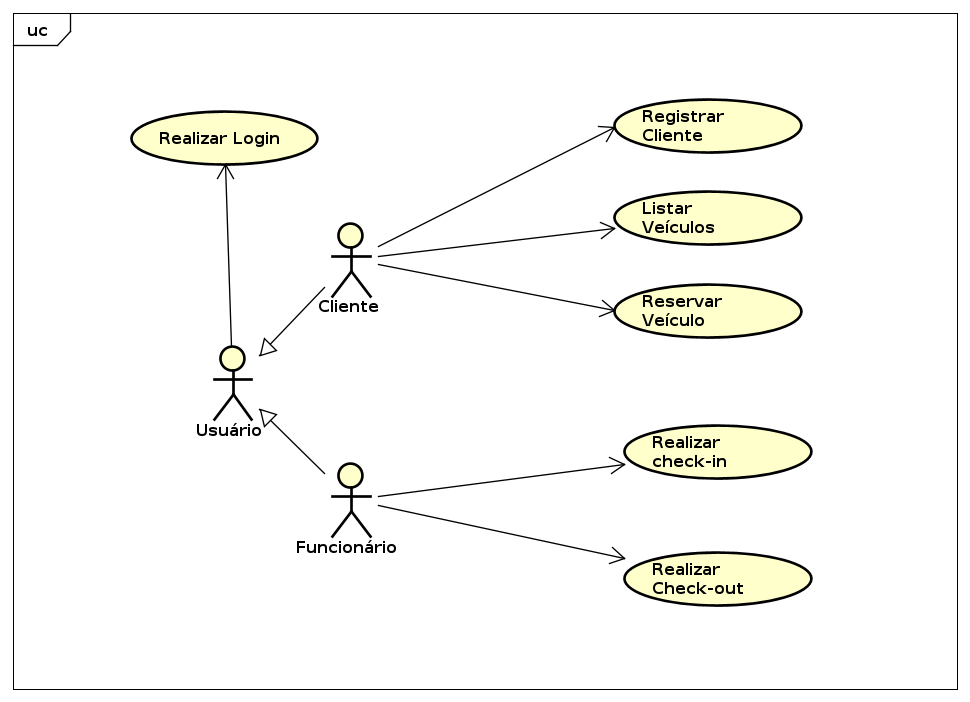
\includegraphics[width=0.9\textwidth]{media/diagrama_usecase.png}
    \legend{Fonte: o autor}
    \label{fig:caso_uso}
\end{figure}

A \autoref{fig:caso_uso} apresenta o diagrama de caso de uso do sistema de locação de veículos. As seções a seguir apresentam um detalhamento dos casos de uso do sistema.

\section{Processo de Desenvolvimento}
\label{section:processo_desenvolvimento}
O processo de desenvolvimento utilizado para construir o sistema de locação de veículos é o \english{Kanban}. Essa metodologia de desenvolvimento ágil é baseada em um quadro de tarefas, no qual cada tarefa é representada por um cartão \cite{gomes2014agile}. O quadro é dividido em colunas que representam o estado atual de cada tarefa. As colunas mais comuns são: \english{To Do}, \english{Doing} e \english{Done}. O quadro é atualizado conforme as tarefas são realizadas. A \autoref{fig:kanban} apresenta um exemplo de quadro \english{Kanban} que é utilizado para mapear as tarefas e medir o progresso do desenvolvimento deste sistema.

\begin{figure}[ht!]
    \centering
    \caption{Exemplo de quadro \english{Kanban}}
    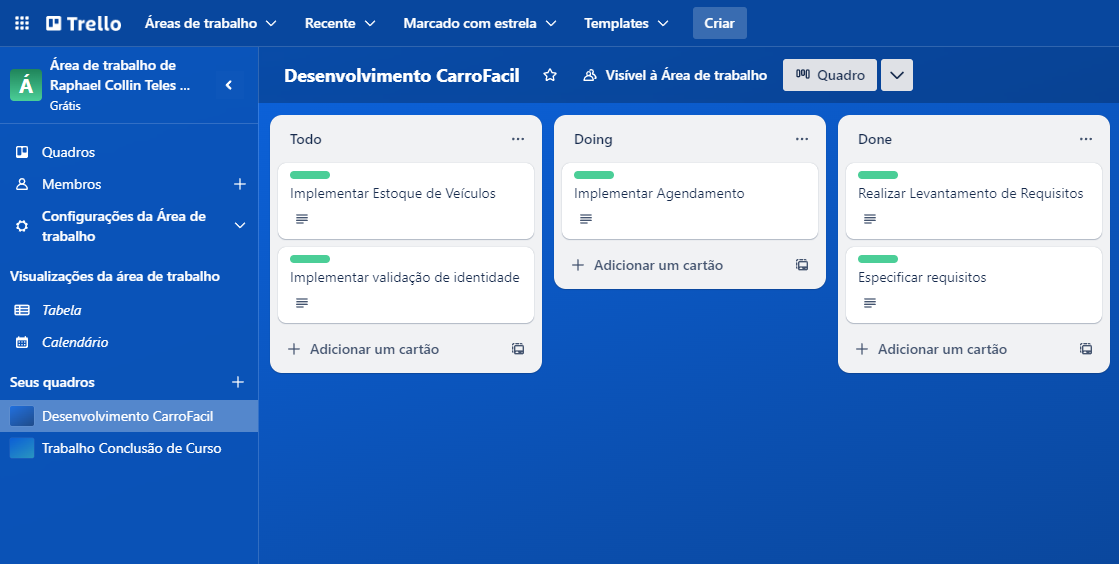
\includegraphics[width=0.9\textwidth]{media/kanban.png}
    \legend{Fonte: o autor}
    \label{fig:kanban}
\end{figure}

\section{Requisitos}
A seguir são apresentados os requisitos do sistema de locação de veículos.
\subsection{Requisitos Funcionais}

\begin{quadro}[H]
    \centering
    \caption{Registrar cliente}
    \label{quad:registrar_cliente}
    \begin{tabular}{|p{1.2in}|p{3.5in}|}
    \hline
    
    \textbf{Caso de uso} & Registrar cliente \\ \hline
    \textbf{Descrição} & Permite que o cliente se cadastre na plataforma. \\ \hline
    \textbf{Ator} & Cliente \\ \hline
    \textbf{Pre-condições} & O cliente ainda não está cadastrado. \\ \hline
    \textbf{Pós-condições} & O cliente é registrado na plataforma.\\ \hline
    \textbf{Cenário Principal} & \begin{enumerate}
        \item O cliente informa o nome, e-mail e senha.
        \item O cliente recebe uma confirmação do cadastro.
    \end{enumerate}  \\ \hline
    \textbf{Fluxo de Exceção} & \begin{enumerate}
        \item Dados inválidos são informados. Nesse caso, o sistema exibe uma mensagem de erro.
        \item Usuário já cadastrado. O sistema também exibe uma mensagem de erro customizada para esse caso.
    \end{enumerate}  \\ \hline
    \end{tabular}
    \fonte{o autor.}
\end{quadro}

O caso de uso do \autoref{quad:registrar_cliente} especifica o registro de um cliente. Esse é o primeiro passo para que um cliente possa realizar uma reserva de veículo.

\begin{quadro}[H]
    \centering
    \caption{Listar veículos}
    \label{quad:listar_veiculos}
    \begin{tabular}{|p{1.2in}|p{3.5in}|}
    \hline
    
    \textbf{Caso de uso} & Listar veículos \\ \hline
    \textbf{Descrição} & Permite que o cliente visualize os veículos disponíveis para locação. \\ \hline
    \textbf{Ator} & Cliente \\ \hline
    \textbf{Pre-condições} & O cliente está autenticado na plataforma. \\ \hline
    \textbf{Pós-condições} & Uma listagem de veículos disponíveis é exibida. \\ \hline
    \textbf{Cenário Principal} & O cliente acessa a página de veículos, onde é possível visualizar os veículos disponíveis. \\ \hline
    
    \end{tabular}
    \fonte{o autor.}
\end{quadro}

O \autoref{quad:listar_veiculos} especifica o processo de listagem de veículos. Esse processo é realizado pelo cliente e permite que ele visualize os veículos disponíveis para aluguel.

\begin{quadro}[H]
    \centering
    \caption{Reservar um veículo}
    \label{quad:reservar_veiculo}
    \begin{tabular}{|p{1.2in}|p{3.5in}|}
    \hline
    
    \textbf{Caso de uso} & Reservar um veículo \\ \hline
    \textbf{Descrição} & Permite que um cliente reserve um veículo por um período de tempo. \\ \hline
    \textbf{Ator} & Cliente \\ \hline
    \textbf{Pre-condições} & O cliente está autenticado na plataforma. \\ \hline
    \textbf{Pós-condições} & Veículo reservado fica indisponível para outros clientes. \\ \hline
    \textbf{Cenário Principal} & \begin{enumerate}
        \item O usuário seleciona o veículo, a data de início e a data de término da locação.
        \item É exibida uma confirmação para o usuário.
    \end{enumerate}  \\ \hline
    \textbf{Fluxo de Exceção} & \begin{enumerate}
        \item O veículo não está mais disponível.
        \item O cliente seleciona um período de tempo indisponível.  
        \item Em ambos os casos, o cliente é alertado sobre o problema.
    \end{enumerate}  \\ \hline
    \end{tabular} 
    \fonte{o autor.}
\end{quadro}

O \autoref{quad:reservar_veiculo} especifica o processo de reserva de um veículo. Esse processo é realizado pelo cliente e permite que ele alugue um veículo por um período de tempo.

\begin{quadro}[H]
    \centering
    \caption{Realizar \english{check-in}}
    \label{quad:realizar_checkin}
    \begin{tabular}{|p{1.2in}|p{3.5in}|}
    \hline
    
    \textbf{Caso de uso} & Realizar \english{check-in} \\ \hline
    \textbf{Descrição} & Permite a realização do check-in da reserva entre o cliente e o funcionário. \\ \hline
    \textbf{Ator} & Funcionário \\ \hline
    \textbf{Pre-condições} & \begin{enumerate}
        \item \O cliente está autenticado na plataforma.
        \item O cliente possui uma reserva criada e seu identificador.
    \end{enumerate} \\ \hline
    \textbf{Pós-condições} & O status da reserva é alterado para em progresso. \\ \hline
    \textbf{Cenário Principal} & O cliente apresenta o identificador da reserva ao funcionário que o insere no sistema para realizar o check-in. \\ \hline
    \textbf{Fluxo de Exceção} & \begin{enumerate}
        \item O check-in para aquela reserva já foi realizado.
        \item O usuário é alertado sobre o problema.
    \end{enumerate}  \\ \hline
    \end{tabular}
    \fonte{o autor.}
\end{quadro}

O caso de uso Realizar \english{check-in} é apresentado no \autoref{quad:realizar_checkin}. Esse caso de uso é realizado pelo funcionário e permite que o cliente retire o veículo reservado.

\begin{quadro}[H]
    \centering
    \caption{Realizar \english{check-out}}
    \label{quad:realizar_checkout}
    \begin{tabular}{|p{1.2in}|p{3.5in}|}
    \hline
    
    \textbf{Caso de uso} & Realizar \english{check-out} \\ \hline
    \textbf{Descrição} & Permite a realização do check-out da reserva entre o cliente e o funcionário. \\ \hline
    \textbf{Ator} & Funcionário \\ \hline
    \textbf{Pre-condições} & \begin{enumerate}
        \item O cliente possui uma reserva em progresso e seu identificador.
        \item O cliente está autenticado na plataforma.
    \end{enumerate} \\ \hline
    \textbf{Pós-condições} & O status da reserva é alterado para concluída. \\ \hline
    \textbf{Cenário Principal} & O cliente retorna o veículo, o funcionário verifica o estado do veículo, e obtém informações sobre a reserva a partir da placa. Por fim, o funcionário finaliza a reserva. \\ \hline
    \textbf{Fluxo de Exceção} & \begin{enumerate}
        \item O \english{check-in} não foi realizado para reserva.
        \item O usuário é alertado sobre o problema.
    \end{enumerate} \\ \hline
    \end{tabular}
    \fonte{o autor.}
\end{quadro}

O \autoref{quad:realizar_checkout} especifica o processo de realização do \english{check-out}. Esse processo é realizado pelo funcionário e permite que o cliente devolva o veículo alugado.

\begin{quadro}[H]
    \centering
    \caption{Listar reservas}
    \label{quad:listar_reservas}
    \begin{tabular}{|p{1.2in}|p{3.5in}|}
    \hline
    
    \textbf{Caso de uso} & Listar reservas \\ \hline
    \textbf{Descrição} & Permite que um cliente visualize as reservas que realizou. \\ \hline
    \textbf{Ator} & Cliente \\ \hline
    \textbf{Pre-condições} & Cliente está autenticado na plataforma. \\ \hline
    \textbf{Pós-condições} & Uma listagem de reservas é exibida. \\ \hline
    \textbf{Cenário Principal} & O cliente acessa a página de reservas, onde é possível visualizar as reservas realizadas. \\ \hline
    
    \end{tabular}
    \fonte{o autor.}
\end{quadro}

O \autoref{quad:listar_reservas} especifica o processo de listagem de reservas. Esse processo é realizado pelo cliente e permite que ele visualize as reservas que realizou.

\begin{quadro}[H]
    \centering
    \caption{Registrar veículo}
    \label{quad:registrar_veiculo}
    \begin{tabular}{|p{1.2in}|p{3.5in}|}
    \hline
    
    \textbf{Caso de uso} & Registrar veículo \\ \hline
    \textbf{Descrição} & Permite que um funcionário registre um novo veículo na plataforma. \\ \hline
    \textbf{Ator} & Funcionário \\ \hline
    \textbf{Pre-condições} & O funcionário está autenticado. \\ \hline
    \textbf{Pós-condições} & O veículo é registrado na plataforma. \\ \hline
    \textbf{Cenário Principal} & \begin{enumerate}
        \item O funcionário informa o tipo, marca, modelo, quilometragem, ano, placa, chassis e a cor do veículo.
        \item O funcionário envia a requisição.
    \end{enumerate}  \\ \hline
    \textbf{Fluxo de Exceção} & \begin{enumerate}
        \item Dados inválidos são informados. Nesse caso, o sistema exibe uma mensagem de erro.
    \end{enumerate}  \\ \hline
    \end{tabular}
    \fonte{o autor.}
\end{quadro}

O \autoref{quad:registrar_veiculo} especifica o processo de registro de um veículo. Esse processo é realizado pelo funcionário e permite que ele registre um novo veículo na plataforma.

\subsection{Requisitos não Funcionais}
Com base na quantidade de clientes atuais e a estimativa de crescimento, bem como suas expectativas quanto ao desempenho do sistema, são definidos os seguintes requisitos não funcionais:
\begin{enumerate}
    \item Os serviços devem garantir a segurança dos dados dos clientes.
    \item O tempo de resposta dos serviços deve ser menor que 2 segundos em 90\% das requisições.
    \item O sistema como um todo deve suportar 100 usuários simultâneos.
    \item As funcionalidades dos serviços devem ser fornecidas através de \acrshort{api}s acessíveis com o protocolo HTTP.
\end{enumerate}

\section{Design}
Para construção de cada microsserviços, é feito uso da \hyperref[section:hexagonal]{Arquitetura Hexagonal}. Essa, por sua vez, separa a aplicação em duas partes principais: núcleo da aplicação e adaptadores. O núcleo da aplicação contém as regras de negócio e os adaptadores são responsáveis por adaptar a aplicação para o mundo externo. Para modelagem do domínio, é utilizado o \english{\acrfull{ddd}}. O \acrshort{ddd} fornece uma estratégia para modelagem do domínio de negócio, diversos padrões para resolver problemas de modelagem recorrentes e facilidade de entendimento e manutenção de código \cite{evans2004ddd}.

Para realização do \english{design} deste projeto, é utilizado a \english{UML}. Especificamente, são criados diagramas de classes com propósito de modelar os tipos de objeto, seus relacionamentos e os serviços que fornecem. Adicionalmente, para detalhamento do fluxo de execução de operações chave, alguns diagramas de sequência são empregados. Além disso, visando fornecer uma visão geral da arquitetura do sistema, o diagrama de contexto de sistema do modelo C4 é utilizado. Esse modelo engloba um conjunto de abstrações hierárquicas e um conjunto de diagramas que fornecem diferentes perspectivas do sistema e que são extremamente úteis para representar a arquitetura de um sistema \cite{c4Model}. 

\section{Implementação}
A implementação desse projeto é feita utilizando a linguagem de programação \english{Java} na versão 17 \cite{java}. Além disso, o \english{framework} \english{Spring Boot} é empregado na construção dos microsserviços. Essa ferramenta fornece uma série de recursos para construção de microsserviços como: injeção de dependências, configuração de banco de dados, configuração de \english{logs}, entre outros \cite{springBoot}. 

São utilizados dois banco de dados para armazenamento dos dados do sistema. O primeiro é um banco de dados relacional, que armazena dados de reservas e veículos. O segundo é um banco de dados não relacional, que armazena dados de usuários. Para o banco de dados relacional, é utilizado o \english{PostgreSQL} \cite{postgreSql}. Para o banco de dados não relacional, foi escolhido o \english{Amazon DynamoDB} \cite{dynamoDb}.

O \english{PostgreSQL} é um sistema de gerenciamento de banco de dados relacional de código aberto. Esse banco de dados é um dos mais populares do mundo, sendo utilizado por diversas empresas, como: \english{Apple}, \english{Spotify}, \english{Netflix}, entre outras \cite{postgreSql}. Trata-se de um banco de dados escalável, confiável, fácil de usar e com suporte a transações \acrshort{acid}.

Por outro lado, o \english{Amazon DynamoDB} é um banco de dados não relacional, que fornece desempenho de milissegundos de um dígito a qualquer escala. Esse banco de dados é totalmente gerenciado, ou seja, não é necessário realizar a configuração de servidores, escalabilidade, replicação, entre outros. Além disso, o \english{Amazon DynamoDB} é um banco de dados sem servidor, ou seja, o usuário paga apenas pelo que utiliza \cite{dynamoDb}.

Para a intercomunicação entre os microsserviços de maneira assíncrona, são utilizados o \english{Amazon Simple Notification System (SNS)} e o \english{Amazon Simple Queue System (SQS)}. O SNS é um serviço de mensagens que permite a publicação e a entrega de mensagens para assinantes ou pontos de extremidade \cite{amazonSns}. Por outro lado, o SQS é um \english{broker} permite que os microsserviços se comuniquem de maneira assíncrona, sem que um microsserviço precise conhecer o outro \cite{amazonSqs}. Além disso, o \english{Amazon SQS} permite que as mensagens sejam armazenadas em uma fila, caso o microsserviço destinatário da mensagem esteja fora do ar. Utilizados em conjunto, essas ferramentas permitem a comunicação assíncrona na forma "um para muitos" entre os microsserviços. Um microsserviço publica uma mensagem em  um tópico do SNS e os microsserviços interessados utilizam uma fila do SQS para consumir essa mensagem.

\section{Validação}
O projeto é desenvolvido com as estratégias \acrfull{tdd} e \acrfull{bdd}. Essas abordagens de desenvolvimento de \english{software} permitem que o código seja desenvolvido de maneira mais confiável e com maior qualidade \cite{barauna2020tdd}. Além disso, o \acrshort{tdd} e o \acrshort{bdd} permitem que o código seja desenvolvido de maneira mais rápida, pois os testes são escritos antes do código.

Três tipos de testes são escritos para validar os requisitos funcionais do sistema: testes unitários, testes de integração e testes de sistema. Os testes unitários são escritos para validar métodos e classes do sistema. Por outro lado, os testes de integração validam a integração entre dois microsserviços e integrações com componentes externos, como banco de dados. Por fim, os testes de sistema são implementados para validar os requisitos do sistema. É importante ressaltar que todos os testes são automatizados utilizando o \english{JUnit} \cite{junit}. O framework \english{Mockito} é utilizado para simular o comportamento de objetos reais \cite{mockito}. Além disso, o \english{Testcontainers} é utilizado para criar contêineres \english{Docker} para os testes de sistema \cite{testcontainers}.

Por outro lado, para validação dos requisitos não funcionais, testes de carga são empregados. O ambiente de execução desses testes é o mesmo de implantação, definido na seção \ref{section:implantacao}. Através da ferramenta Gatling \cite{gatling}, a bateria de testes consiste de 100 usuários executando operações simultâneas por um período de 30 minutos. São avaliados o tempo de resposta, a utilização da CPU, o consumo de memória e a quantidade erros. Os resultados obtidos são comparados com o \autoref{quad:metricas_comparacao}. Cada operação possui as seguintes etapas: registrar um novo veículo, cadastrar um cliente, realizar uma reserva, realizar o \english{check-in} e realizar o \english{check-out}.

Após a execução dos testes de carga, os resultados obtidos são avaliados e comparados com os requisitos não funcionais. Dessa forma, um relatório é produzido com uma análise gráfica e numérica.

\begin{quadro}[H]
    \centering
    \caption{Métricas de comparação}
    \label{quad:metricas_comparacao}
    \begin{tabular}{|p{1.2in}|p{3.5in}|}
    \hline
    
    \textbf{Métrica} & \textbf{Alvo} \\ \hline
    Tempo de resposta & <= 2 s em 90\% das requisições. \\ \hline
    Utilização da CPU & <= 70\% durante toda a execução. \\ \hline
    Consumo de memória & <= 70\% durante toda a execução. \\ \hline
    Quantidade de erros & <= 1\% das requisições. \\ \hline

    \end{tabular}
    \fonte{o autor.}
\end{quadro}

Os parâmetros descritos no \autoref{quad:metricas_comparacao} foram definidos pelo autor com base em experiências anteriores de desenvolvimento de sistemas similares no ambiente corporativo, juntamente com a recomendação do orientador.

\section{Implantação}
\label{section:implantacao}
O sistema é implantado na nuvem da \english{\acrfull{aws}}. A \acrshort{aws} é uma plataforma de computação em nuvem que oferece mais de 200 serviços completos de \english{data centers} em todo o mundo \cite{aws}. Esses serviços incluem computação, armazenamento, banco de dados, \english{networking}, \english{analytics}, \english{machine learning}, inteligência artificial, \english{Internet of Things}, segurança, entre outros.

Cada microsserviço é implantado em um \english{container} \english{Docker}. Essa tecnologia permite que os microsserviços sejam executados de maneira isolada, sem que um microsserviço interfira no outro. Além disso, o \english{Docker} permite que os microsserviços sejam executados em qualquer ambiente, sem que seja necessário realizar alterações no código \cite{docker}. O serviço \english{Amazon ECS} é utilizado para orquestrar os \english{containers} \english{Docker}. Esse serviço permite que os \english{containers} sejam executados em um ambiente de produção de maneira escalável e confiável \cite{amazonEcs}. Ao todo, serão utilizadas 5 \english{tasks} (uma para cada microsserviço). Cada \english{task} possui 2 CPUs e 4 GB de memória RAM.

Dois \english{clusters} do \english{PostgreSQL} com o auxílio do serviço \english{Amazon RDS} são utilizados \cite{postgreSql}. Um para o serviço de estoque e outro para o serviço de reservas. Com a arquitetura de microsserviços, é essencial o isolamento das bases de dados. Além disso, três tabelas do \english{Amazon DynamoDB} são utilizadas para armazenamento de informações de usuários, clientes e funcionários. Da mesma forma, um tópico do SNS para reservas e um fila SQS que consome informações de reservas e mantém um contador de reservas por cliente são utilizados.

Para a orquestração e automatização do provisionamento e configuração da infraestrutura, é feito uso da ferramenta \english{Terraform}. Essa ferramenta permite que a infraestrutura seja definida como código, ou seja, é possível definir a infraestrutura utilizando uma linguagem de programação \cite{terraform}. Além disso, o \english{Terraform} permite que a infraestrutura seja provisionada e configurada de maneira automatizada.
